\section{Results} \label{results-section}
Having established our research design, this section presents the results of the analyses conducted. First, we describe the stock returns and investor sentiment data, while also looking at the types of companies found in S\&P 500 and DJIA, and the types of investors using the platform StockTwits. Then, we study the relationship between trading volume and number of sentiment messages, and the correlations between different investor sentiment measures, both traditional and modern. This allows us to better understand when users express their sentiment and whether this behaviour is influenced by higher volatility. Finally, the results of the third level of our research are presented, where we test what is the relationship between modern investor sentiment measures and subsequent stock returns.

\subsection{Descriptive Statistics}
Descriptive statistics present information about the data used and summarises its important features. In the quantitative analysis, we are most interested in the mean, the standard deviation and the number of observations of the dataset in order to have an indication of data variability. These features are presented in the following subsections.

\subsubsection{Dependent Variable: Stock Returns}
Table~\ref{tab:table4} below summarizes the monthly and weekly returns of \$SPY and \$DIA for the period 01/01/2014 - 31/12/2016. The means of returns are slightly positive and almost identical for both ETFs. Surprisingly, \$DIA has higher standard deviation both on a monthly and weekly basis, even though it mostly consists of large companies. S\&P500 presents a more diversified portfolio which in turn might reduce the variability between returns. An interesting contrast is the existence of more extreme minimum and maximum values for \$DIA compared to \$SPY.


\sbox\tempbox{%
\begin{tabular}{@{}lllll@{}}
\toprule
        & \multicolumn{2}{l}{\textbf{Monthly}} & \multicolumn{2}{l}{\textbf{Weekly}} \\ \midrule
        & \$SPY             & \$DIA            & \$SPY            & \$DIA            \\
Mean    & 0.0087            & 0.0086           & 0.0016           & 0.0015           \\
Std Dev & 0.0324            & 0.0339           & 0.0190           & 0.0192           \\
Min     & -0.0737           & -0.0765          & -0.1017          & -0.1024          \\
Max     & 0.0884            & 0.0903           & 0.0566           & 0.0606           \\
N       & 36                & 36               & 157              & 157              \\ \bottomrule
\end{tabular}%
}
\setlength\templen{\wd\tempbox}
\begin{table}[h]
\centering
\usebox{\tempbox}\\[3pt]
\parbox{\the\templen}{\small This table shows descriptive statistics for the weekly and monthly returns of \$SPY and \$DIA ETFs.}
\caption{Descriptive Statistics of Stock Returns}
\label{tab:table4}
\end{table}


\subsubsection{Description of Companies in S\&P 500 and DJIA}
Dow Jones Industrial Average consists of 30 companies, which are large, traditional American corporations with long history. The companies in S\&P500 are picked by the S\&P committee and are generally the 500 largest publicly traded companies on the US market. Therefore, S\&P 500 is more diverse and includes also companies with lower market capitalization. Figures~\ref{fig:figure2} and~\ref{fig:figure3} below show both indices divided by industry.

\begin{figure}[ht]
\centering
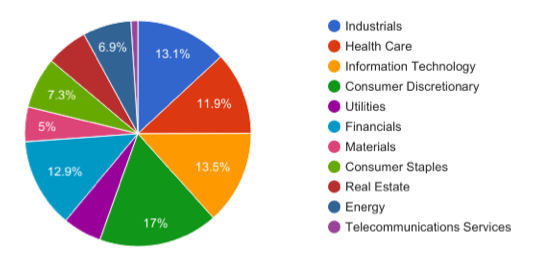
\includegraphics[width=0.75\textwidth]{figures/figure2.png}
\caption{\label{fig:figure2}Industries of Companies in S\&P 500}
\end{figure}

\begin{figure}[ht]
\centering
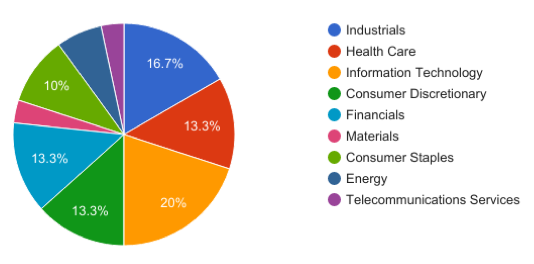
\includegraphics[width=0.75\textwidth]{figures/figure3.png}
\caption{\label{fig:figure3}Industries of Companies in DJIA}
\end{figure}

The graphs visualize that both S\&P 500 and DJIA have a wide spread of companies from all major industries. Our research is therefore not limited to a specific branch but allows generalization to different industries on the US market.

\newpage

\subsubsection{Independent Variable: Investor Sentiment}
As mentioned before in section~\ref{research_strategy}, we gather investor sentiment data from three data sources, which are statistically described in this section.
\par
Table~\ref{tab:spy-descriptives} below summarizes the descriptive statistics of investor sentiment measures for \$SPY. The sentiment level is defined as the percentage of bullish posts; therefore, it is in the interval [0,1].

\sbox\tempbox{%
  \begin{tabular}{crrrrrrr}
    \multicolumn{2}{c}{\textbf{\$SPY}} & \multicolumn{3}{c}{\textbf{Monthly}} & \multicolumn{3}{c}{\textbf{Weekly}} \\
    \toprule
    \multicolumn{2}{c}{Source} & \multicolumn{2}{c}{PsychSignal} & \multicolumn{1}{c}{StockTwits} & \multicolumn{2}{c}{PsychSignal} & \multicolumn{1}{c}{StockTwits} \\
    \midrule
    \multicolumn{2}{c}{Database} & \multicolumn{1}{c}{\specialcell{PS:\\ Agg.}} & \multicolumn{1}{c}{\specialcell{PS: \\StockTwits}} & \multicolumn{1}{c}{StockTwits} & \multicolumn{1}{c}{\specialcell{PS: \\Agg.}} & \multicolumn{1}{c}{\specialcell{PS: \\StockTwits}} & \multicolumn{1}{c}{StockTwits} \\
    \midrule
    \multirow{5}[0]{*} {\specialcell{Absolute \\ Sentiment}}
     & Mean  & 0.5991 & 0.5948 & 0.4181 & 0.6009 & 0.5962 & 0.4184 \\
          & Std dev & 0.0464 & 0.0197 & 0.0623 & 0.0637 & 0.0330 & 0.0922 \\
          & Min   & 0.4944 & 0.0541 & 0.2701 & 0.3660 & 0.5210 & 0.2161 \\
          & Max   & 0.7535 & 0.6334 & 0.5199 & 0.8198 & 0.6905 & 0.6540 \\
          & N     & 3613956 & 1418685 & 204547 & 3613956 & 1418685 & 204547 \\
    \multirow{5}[0]{*} {\specialcell{Change in \\ Sentiment}} & Mean  & 0.0066 & 0.0026 & 0.0157 & 0.0102 & 0.0025 & 0.4518 \\
          & Std dev & 0.0949 & 0.0412 & 0.1781 & 0.1449 & 0.0691 & 0.1695 \\
          & Min   & -0.0204 & -0.0636 & -0.2523 & -0.4484 & -0.2290 & 0.0667 \\
          & Max   & 0.2610 & 0.0851 & 0.5465 & 0.7017 & 0.1692 & 10,000 \\
          & N     & 3613956 & 1418685 & 204547 & 3613956 & 1418685 & 204547 \\
          
          \bottomrule
    \end{tabular}%
}
\setlength\templen{\wd\tempbox}
\begin{table}[htbp]
\centering
\usebox{\tempbox}\\[3pt]
\parbox{\the\templen}{\small This table shows the descriptive statistics of investor sentiment data of ETF \$SPY for the studied period. Sentiment data is aggregated both on weeks and months, and the table includes the description of all three datasets.}
\caption{Descriptive statistics for investor sentiment of \$SPY}%
\label{tab:spy-descriptives}%
\end{table}%


For both investor sentiment measures provided by PsychSignal we were able to collect large amounts of data points, precisely between 1.5 million and 3.6 million. Messages with sentiment label on StockTwits, thereby being categorised as direct measurement, were approximately 200,000. The means of the bullish percentages of \$SPY posts from both PS:Aggregated and PS:StockTwits are very similar, close to 60\%. Monthly values stay close to the mean, whereas the minimum and maximum values of the weekly sentiment have a larger spread. The minimum sentiment measure from PS:Aggregated of \$SPY is 36.6\%, while the maximum is 81,98\%.
\par
Looking for differences between direct sentiment measure on StockTwits and the data provided by PsychSignal, the first major noticeable difference is the large difference between the means of bullish percentage. The bullish percentage from StockTwits is only about 41.81\% (both for months and weeks), compared to the 60\% from PS:StockTwits. As a result, we can conclude that users are more likely to provide bearish labels with their messages or the NLP algorithm is skewed towards positivity. Moreover, this also implies that unlabelled messages can be evaluated often as bullish by PsychSignal's NLP. Which measure shows the strongest relationship to subsequent stock returns will be discussed in section~\ref{sentiment-measure-discussion}. The correlation between the measurements obtained from PsychSignal and StockTwits are analysed in section~\ref{correlation-sentiments}. Table~\ref{tab:dia-descriptives} below summarizes the descriptive statistics on investor sentiment measures for \$DIA.

\sbox\tempbox{%
    \begin{tabular}{crrrrrrr}
    \multicolumn{2}{c}{\textbf{\$DIA}} & \multicolumn{3}{c}{\textbf{Monthly}} & \multicolumn{3}{c}{\textbf{Weekly}} \\
    \toprule
    \multicolumn{2}{c}{Source} & \multicolumn{2}{c}{PsychSignal} & \multicolumn{1}{c}{StockTwits} & \multicolumn{2}{c}{PsychSignal} & \multicolumn{1}{c}{StockTwits} \\
    \midrule
 	\multicolumn{2}{c}{Database} & \multicolumn{1}{c}{\specialcell{PS: \\Agg.}} & \multicolumn{1}{c}{\specialcell{PS: \\StockTwits}} & \multicolumn{1}{c}{StockTwits} & \multicolumn{1}{c}{\specialcell{PS: \\Agg.}} & \multicolumn{1}{c}{\specialcell{PS: \\StockTwits}} & \multicolumn{1}{c}{StockTwits} \\
    \midrule
    \multirow{5}[1]{*}{\specialcell{Absolute \\sentiment}} & Mean  & 0.6012 & 0.6096 & 0.4377 & 0.6194 & 0.6124 & 0.4518 \\
          & Std dev & 0.1273 & 0.0531 & 0.1003 & 0.1516 & 0.0802 & 0.1695 \\
          & Min   & 0.2824 & 0.4943 & 0.2793 & 0.1603 & 0.4268 & 0.0667 \\
          & Max   & 0.7474 & 0.7233 & 0.6932 & 0.8765 & 0.8718 & 1000 \\
          & N     & 437618 & 65747 & 5542  & 437618 & 65747 & 5542 \\
    \multirow{5}[0]{*}{\specialcell{Change in \\sentiment}} & Mean  & 0.0701 & 0.0080 & 0.0322 & 0.0881 & 0.0131 & 0.1638 \\
          & Std dev & 0.4167 & 0.1246 & 0.3009 & 0.5322 & 0.1690 & 0.7603 \\
          & Min   & -0.5099 & -0.1923 & -0.3710 & -0.6935 & -0.3615 & -0.7537 \\
          & Max   & 13977 & 0.3306 & 0.7279 & 30471 & 0.5378 & 52,473 \\
          & N     & 437618 & 65747 & 5542  & 437618 & 65747 & 5542 \\
          \bottomrule
    \end{tabular}%
}
\setlength\templen{\wd\tempbox}
\begin{table}[htbp]
\centering
\usebox{\tempbox}\\[3pt]
\parbox{\the\templen}{\small This table shows the descriptive statistics of investor sentiment data of ETF \$DIA for the studied period. Sentiment data is aggregated both on weeks and months, and the table includes description of all three datasets.}
\caption{Descriptive statistics for investor sentiment of \$DIA}
\label{tab:dia-descriptives}%
\end{table}%



\par
The numbers follow a similar pattern as described for ETF \$SPY. There is less activity for \$DIA on social media than for \$SPY, resulting in fewer data points available. However, with a minimum of 30 messages per week there is enough data available to draw conclusions about the investor sentiment. The most striking difference between both PsychSignal data sources and StockTwits is again a lower bullish percentage if users directly state their sentiment. Therefore, lower sentiment when explicitly asked seems to generally apply for most stocks/indexes.

\subsubsection{Type of investors on investment platform StockTwits}
StockTwits allows users to define their Experience, Investing Approach and Holding Period. Below are the distribution graphs of StockTwits users based on these three variables. StockTwits users have mainly intermediate experience, with focus on short term investments and growth, technical and momentum strategies.
\par
While we do not differentiate in our research between investor groups, the information about the distribution carries value because it shows which types of investors leave their opinions on social media. The distributions for each investor distinction are even. The investing approaches from traders range from growth to value (Figure ~\ref{fig:figure4}), with most traders applying a technical approach. This is not surprising, since PsychSignal and StockTwits is used by traders who are interested in maximizing their returns by applying quantitative strategies and algorithms. 

\begin{figure}[ht]
\centering
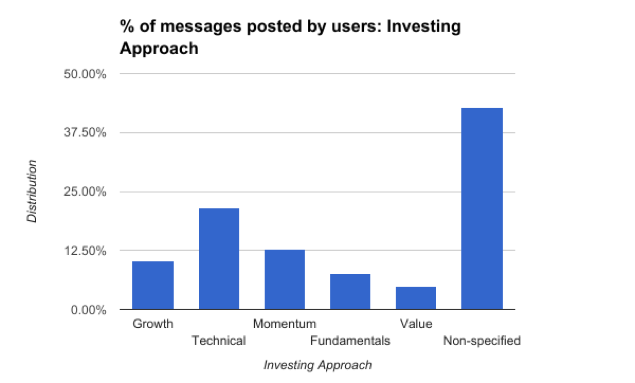
\includegraphics[width=0.6\textwidth]{figures/figure4.png}
\caption{\label{fig:figure4}Investing Approach}
\end{figure}

The traders' experience as classified by themselves is mostly intermediate (30\%), and the novices and professional investors have almost equal proportions (each approximately 15\%). Therefore, our research cannot be categorized by investor types, but is more an indicator of sentiment across all trader groups.

\begin{figure}[ht]
\centering
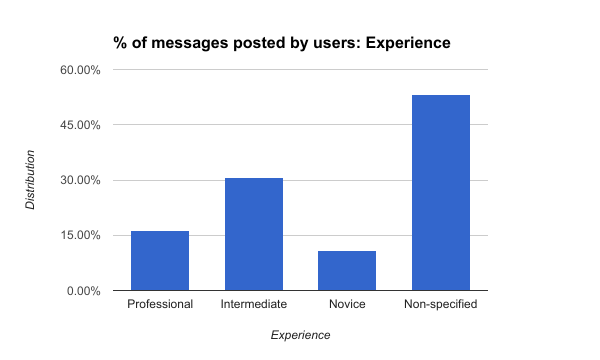
\includegraphics[width=0.6\textwidth]{figures/figure5.png}
\caption{\label{fig:figure5}Trader Experience}
\end{figure}

Lastly, we looked at the holding period of the traders posting messages on StockTwits. Once more, traders apply a range of different methods, from swing traders to long-term investors. 

\begin{figure}[ht]
\centering
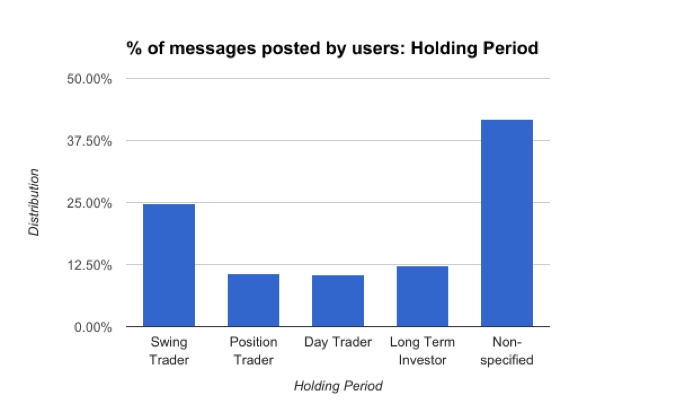
\includegraphics[width=0.6\textwidth]{figures/figure6.png}
\caption{\label{fig:figure6}Holding Period}
\end{figure}

Conclusively, our results will indicate relationships for aggregates of different investor types and investment approaches. To conduct research that evaluates the relationship between stock-specific sentiment and returns of that stock and also differentiate between investor groups, more data points are required. Separating by investor groups would cause the amount of data points available per week to fall significantly. 

\subsection{Relationship between Trading Volume and number of sentiment messages}
In previous researches of social media investor sentiment and sentiment derived via NLP algorithms and its relationship to stock returns (Bollen et al. 2011, Rao et al. 2012, Chen et al. 2013 or Skuza et al. 2015), the authors outlined that increased trading volume is positively correlated with increased number of sentiment messages. We run the tests for both \$SPY and \$DIA and StockTwits messages to see whether this holds true in our data. The correlation scatter plots 
are Figure~\ref{fig:figure7} and Figure~\ref{fig:figure8} respectively.

As expected we can see a strong positive relationship between the trading volume and the number of StockTwits messages for \$SPY and \$DIA. This notion highlights that when a financial instrument is traded in abnormal volumes, people tend to share more sentiment and more opinions about its development. This shows that the investor's react strongly towards high trading volumes (usually after an important event occurs) and share sentiment. It implies that the sentiment measured is strongly influenced by recent events and might not reflect primarily the opinion of investors based on thorough analysis in the long term. This contrasts with the way how AAII measures investor sentiment, where the investors share their opinion about the market in 6-month lag. These results seem to be consistent with the nature of individual investors, especially those, who focus on shorter-term trades using growth, technical or momentum strategies. Figure~\ref{fig:figure6} shows that these types of investors are prevalent on StockTwits. Thus, we expect that investor sentiment measured by StockTwits will be influencing stock returns in near term.

\newpage

\begin{figure}[h]
\centering
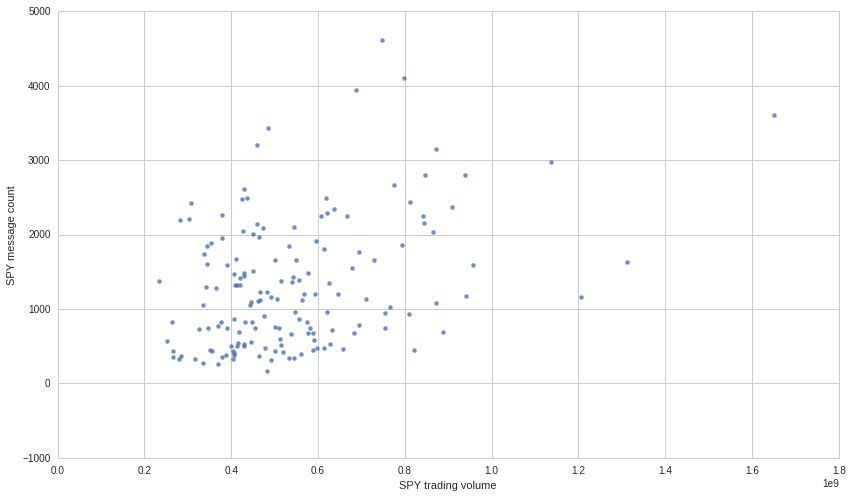
\includegraphics[width=0.8\textwidth]{figures/figure7.png}
\caption{\label{fig:figure7}Correlation Trading Volume and posts about \$SPY. p-value = 0.0000; coefficient =  0.3747 }
\end{figure}

\begin{figure}[h]
\centering
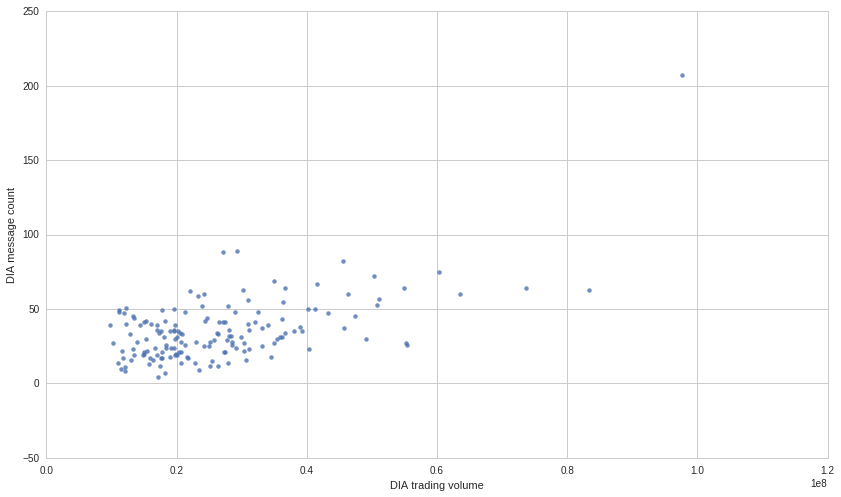
\includegraphics[width=0.8\textwidth]{figures/figure8.png}
\caption{\label{fig:figure8}Correlation Trading Volume and posts about \$DIA. p-value = 0.0000; coefficient = 0.5927}
\end{figure}

\newpage

\subsection{Correlation analyses between investor sentiment measures} \label{correlation-sentiments}
In this section, we look at levels 1 and 2 of our research, where we compare the modern sentiment measures with the traditional sentiment survey employed by AAII. Furthermore, we analyse the degree of association between different modern sentiment measures.

\subsubsection{Modern sentiment measures}
As seen in the descriptive statistics, there exist differences in the investor sentiment measures that we employ in our research. We compare \$SPY and \$DIA sentiments from the three databases both on weekly and monthly basis. All pairs investigated, except for two instances, exhibit relationship at the 1\% significance level with a coefficient of correlation between 0.21 and 0.72. The table with all the results can be found in Appendix, Table~\ref{tab:appendix2}.
\par
The highest coefficient is between monthly \$SPY from PS:StockTwits and monthly \$DIA from PS:StockTwits. Interestingly, the same pair, but with direct sentiment measure from StockTwits is not significantly correlated. This result follows the notion from descriptive statistics: the standard deviation of StockTwits measure is higher than PS:StockTwits.
\par
For \$SPY sentiment, StockTwits PS:StockTwits and StockTwits correlate at 1\% confidence level (0.55). For \$DIA, this relationship is similar, with coefficient of 0.57 at 1\% level.

\subsubsection{AAII and StockTwits direct investor sentiment measure}
To check how the contemporary investor sentiment measures compare to the more traditional ones, we analysed the connection between AAII and direct StockTwits sentiment measure through a correlation analysis.

\begin{figure}[ht]
\centering
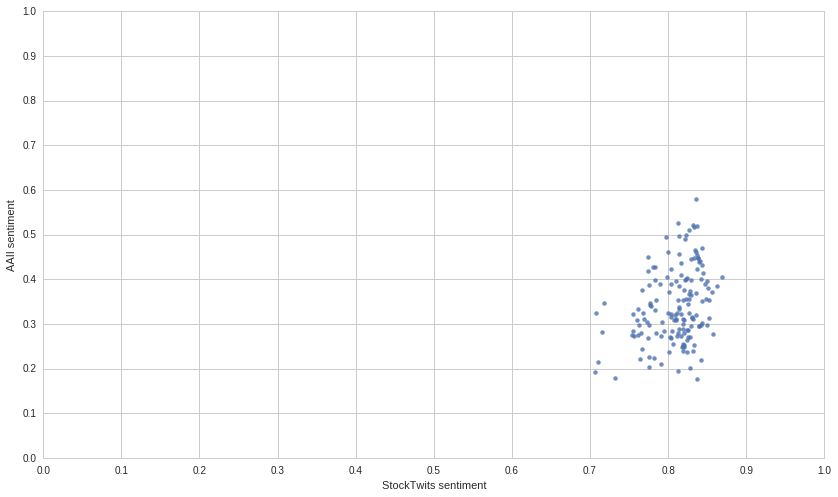
\includegraphics[width=1\textwidth]{figures/corrST-AAII.png}
\caption{\label{fig:figure9}Correlation StockTwits and AAII ($r=0.3119$)}
\end{figure}

The relationship is significant (p-value < 0.000) with a correlation coefficient of 0.3119. This shows an existent, but weak-moderate correlation between these two sentiment measures. In comparison, according to Brown and Cliff (2004), AAII and Investor Intelligence correlate significantly with a coefficient of 0.47. We can conclude that the new, social media and big data approach correlates with traditional investment sentiment measures via surveys only moderately. One more thing which becomes clear from correlation analysis is the much stronger average bullishness sentiment on StockTwits as compared to the AAII surveys. One of the next steps is to analyse whether one of the measurement types carries more value in predicting future stock performance, discussed in section~\ref{discussion-section}.

\subsubsection{AAII and PsychSignal indirect investor sentiment measures}
Following the analysis of investor sentiment between two direct measures (AAII and StockTwits), we want to investigate how the modern indirect measures from PsychSignal correlate with the traditional AAII direct measure. Since AAII sentiment survey is a market-wide sentiment measure, the indirect measures employed from PsychSignal need to reflect a market-wide sentiment as well. For this reason, the datasets used have included all available sentiment data points.
\par
First, we run correlation test between PS:StockTwits and AAII, which shows highly significant results with p-value ${\approx}$ 0.000, and a coefficient of correlation of 0.3963. This coefficient implies a weak-moderate positive relationship between the two sentiment measures and shows that PS:StockTwits dataset correlates with AAII to some extent. Figure~\ref{fig:figure10} shows the scatter plot for this relation between variables.

\begin{figure}[ht]
\centering
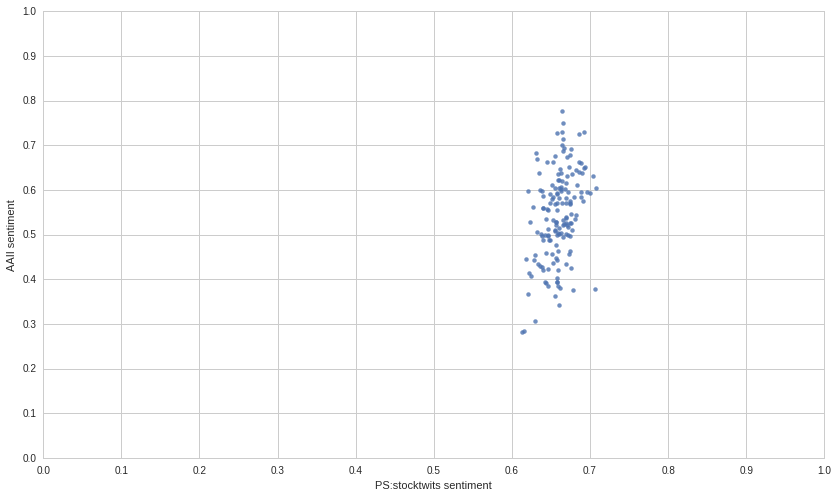
\includegraphics[width=1\textwidth]{figures/figure10.png}
\caption{\label{fig:figure10}Correlation PS:StockTwits and AAII (\textit{r}=0.3963)}
\end{figure}

The second correlation test is made between PS:Aggregated and AAII. Although the results are significant at the 10\% level (p-value = 0.0867), the Pearson correlation coefficient equals only 0.1372, indicating that there is a very weak association. This weak relationship can be observed in figure~\ref{fig:figure11}.

\begin{figure}[ht]
\centering
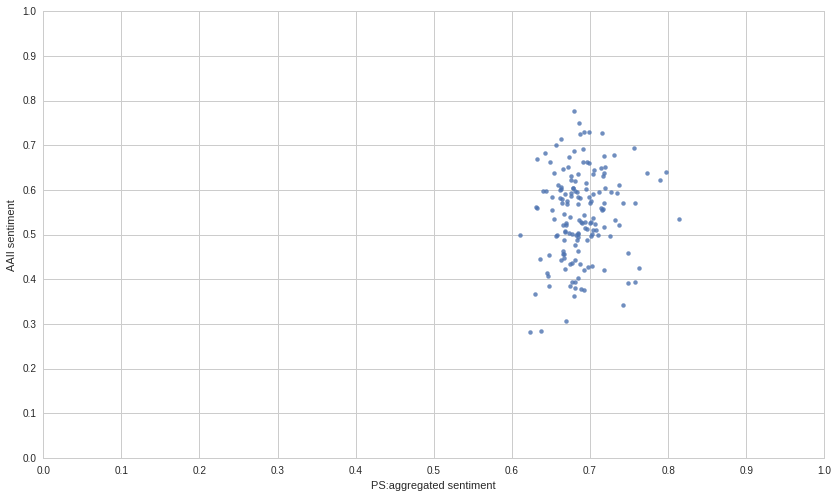
\includegraphics[width=1\textwidth]{figures/figure11.png}
\caption{\label{fig:figure11}Correlation PS:Aggregated and AAII (\textit{r}=0.1372)}
\end{figure}

A comparison of the two scatter plots clearly shows the difference between correlation coefficients. One of the explanations for this variation in results is given by the fact that dataset PS:Aggregated provides the results of an analysis of more messages than PS:StockTwits does, since the former includes Twitter posts in the analysis. This difference might reduce the overall bullishness feature or enhance the bearishness of sentiment. The previous results provide the basis of another correlation analysis between the market-wide sentiment measure given by the two PsychSignal datasets. Thus, running correlation analysis between PS:Aggregated and PS:StockTwits, the results are significant, with Pearson coefficient of 0.4627. Hence, this moderate relationship shows that these two datasets provide dissimilar sentiment measures.

\subsection{The relationship between modern investor sentiment measures and subsequent stock returns}

With significant correlations present between traditional and modern investor sentiment measures, we turn our attention to research level 3, which investigates the main hypothesis of the paper. In this part, we want to test whether periods with higher levels of investor sentiment are followed by periods with negative stock returns and vice versa. To investigate this relationship, we analyse the connection between subsequent stock returns and the three investor sentiment measures databases mentioned before: (1) StockTwits, (2) PS:StockTwits and (3) PS:Aggregated.
\par
We run univariate regressions which differ in lag, monthly or weekly periods and absolute value or the change in sentiment as the independent variable. All these factors have been highlighted in previous research as variables which produce different results. Since the research in the modern sentiment measures is new, our main goal is to establish basic relationships and thus we test for all these factors. The most significant outcomes are highlighted below, while all regression analyses results can be found in Appendix, Table~\ref{tab:appendix}.

\subsubsection{StockTwits - StockTwits direct sentiment measure}

\begin{center}

\itshape{
$H_{1a}:$ Investor Sentiment measured directly on StockTwits does not affect subsequent stock returns in S\&P 500.


$H_{1b}:$ Investor Sentiment measured directly on StockTwits does not affect subsequent stock returns in DJIA.
}

\end{center}

Both \$DIA and \$SPY have a significant (at 5\%) negative relationship between absolute StockTwits direct sentiment measured on weekly basis with 1 week lag. The effect sizes are -0.0198 and -0.0328, respectively. This means that 1\% increase in the sentiment measure leads to decrease of 0.00198 pp in \$DIA stock return. \$SPY exhibits a significant (5\%) result for the monthly period with 1 month lag. 
\par
Measuring the change of sentiment did not yield any significant results, except for \$DIA monthly with 3-month lag (10\% confidence level; effect size: 0.032). This relationship is positive, in contrast to previous results. Results indicate that the monthly change in sentiment is positively related to increase in returns on a longer term (3 months).

% Table generated by Excel2LaTeX from sheet 'stocktwits direct'
\sbox\tempbox{%
  \begin{tabular}{lccccrrr}
  & Type  & Agg.  & Database & Lag   & \multicolumn{1}{c}{Slope} & \multicolumn{1}{c}{p-value} & \multicolumn{1}{c}{$R^2$} \\
  \toprule
  \rowcolor[rgb]{ .949,  .949,  .949} \$SPY & Absolute & Weekly & StockTwits & 1-week & -0.0328** & 0.0367 & 2.80\% \\
  \rowcolor[rgb]{ .949,  .949,  .949} \$SPY & Absolute & Weekly & StockTwits & 6-week & -0.0253 & 0.1069 & 2.80\% \\
  \$DIA & Absolute & Weekly & StockTwits & 1-week & -0.0199** & 0.0283 & 3.08\% \\
  \rowcolor[rgb]{ .949,  .949,  .949} \$SPY & Absolute & Monthly & StockTwits & 1-month & -0.1531** & 0.0479 & 11.02\% \\
  \$DIA & Change & Monthly & StockTwits & 3-month & 0.0320* & 0.0612 & 10.22\% \\
  \bottomrule
  \end{tabular}%
}
\setlength\templen{\wd\tempbox}
\begin{table}[htbp]
\centering
\usebox{\tempbox}\\[3pt]
\parbox{\the\templen}{\small This table presents the results of the regression analysis between investor sentiment from StockTwits dataset and stock returns of \$SPY and \$DIA, aggregated weekly and monthly with different time lags. The asterisks mark the level of significance: ***: 0.01, **: 0.05, *: 0.10}
\caption{Results Regression of StockTwits direct sentiment and Stock Returns}
\label{tab:stocktwits-direct}%
\end{table}%


\subsubsection{PS: StockTwits - StockTwits indirect sentiment measure determined by PsychSignal}

\begin{center}

\itshape{
$H_{2a}:$ Investor Sentiment measured indirectly on StockTwits does not affect subsequent stock returns in S\&P 500.

$H_{2b}:$ Investor Sentiment measured directly by StockTwits does not affect subsequent stock returns in DJIA.
}

\end{center}

In contrast with the previous findings, absolute weekly \$SPY sentiment is not negatively related with 1 week lag in stock returns. \$DIA stays significant (10\%) on this level and the effect size increases to -0.0339.
\par
On the one hand, \$DIA weekly is significant for change in sentiment,both for 4 and 8 period lags. On the other hand, \$SPY is significant for change in sentiment in monthly periods with lag 2. For absolute values, 3-month lag is significant again with positive effect size. Also, other results, even not significant show positive slopes for the 3-month lag – the longest term what we analysed.
\par
The other significant results, \$DIA for 4 and 8-week lags, also exhibit positive relationships. Both are, as well, more long term. In contrast, \$SPY 2-month lag shows a negative relationship at 5\% level with a coefficient -0.2744.

% Table generated by Excel2LaTeX from sheet 'stocktwits indirect'
\sbox\tempbox{%
    \begin{tabular}{lccccrrr}
          & Type  & Agg.  & Database & Lag   & \multicolumn{1}{c}{Slope} & \multicolumn{1}{c}{p-value} & \multicolumn{1}{c}{$R^2$} \\
    \toprule
    \rowcolor[rgb]{ .949,  .949,  .949} \$SPY & Absolute & Weekly & PS: StockTwits & 1-week & -0.0543 & 0.2395 & 0.89\% \\
    \$DIA & Absolute & Weekly & PS: StockTwits & 1-week & -0.0339* & 0.0747 & 2.03\% \\
    \rowcolor[rgb]{ .949,  .949,  .949} \$SPY & Absolute & Monthly & PS: StockTwits & 3-month & 0.0487* & 0.0661 & 9.59\% \\
    \rowcolor[rgb]{ .949,  .949,  .949} \$SPY & Change & Monthly & PS: StockTwits & 2-month & -0.2744** & 0.0335 & 12.98\% \\
    \$DIA & Change & Weekly & PS: StockTwits & 4-week & 0.0146* & 0.0970 & 1.78\% \\
    \$DIA & Change & Weekly & PS: StockTwits & 8-week & 0.0183** & 0.0402 & 2.71\% \\
    \bottomrule
    \end{tabular}%
}
\setlength\templen{\wd\tempbox}
\begin{table}[htbp]
\centering
\usebox{\tempbox}\\[3pt]
\parbox{\the\templen}{\small This table shows the results of the regression tests between investor sentiment from PS:StockTwits and stock returns of \$SPY and \$DIA, aggregated weekly and monthly with different time lags. The asterisks are related to the level of significance: ***: 0.01, **: 0.05, *: 0.10}
\caption{Results Regression StockTwits NLP sentiment and Stock Returns}
\label{tab:stocktwits-indirect}%
\end{table}%


\subsubsection{PS:Aggregated - Aggregated Twitter and StockTwits indirect sentiment determined by PsychSignal}

\begin{center}

\itshape {
$H_{3a}:$ Investor Sentiment measured indirectly on StockTwits and Twitter does not affect subsequent stock returns in S\&P 500.

$H_{3b}:$ Investor Sentiment measured directly by StockTwits and Twitter does not affect subsequent stock returns in DJIA.
}

\end{center}

For the PS:Aggregated results, neither \$SPY or \$DIA exhibit significant results for the 1 week lag. However, we see a similar pattern in positive relationships between sentiment measures and stock returns for 12-week lag. \$DIA, both absolute and change in investor sentiment, shows this relationship. 
Conversely, for \$SPY both absolute and change sentiment measures are significant on weekly aggregate with 6-week lag. \$DIA follows this pattern as well for absolute weekly sentiment – all these relationships are negative.

% Table generated by Excel2LaTeX from sheet 'twitter+stocktwits indirect'
\sbox\tempbox{%
    \begin{tabular}{lccccrrr}
          & Type  & Agg.  & Database & Lag   & \multicolumn{1}{c}{Slope} & \multicolumn{1}{c}{p-value} & \multicolumn{1}{c}{R\^2} \\
    \toprule
    \rowcolor[rgb]{ .949,  .949,  .949} \$SPY & Absolute & Weekly & PS: Aggregate & 6-week & -0.0448* & 0.0599 & 2.27\% \\
    \$SPY & Change & Weekly & PS: Aggregate & 6-week & -0.0280*** & 0.0076 & 4.54\% \\
    \rowcolor[rgb]{ .949,  .949,  .949} \$DIA & Absolute & Weekly & PS: Aggregate & 6-week & -0.0187* & 0.0628 & 2.22\% \\
    \rowcolor[rgb]{ .949,  .949,  .949} \$DIA & Absolute & Weekly & PS: Aggregate & 12-week & 0.0240** & 0.0152 & 3.74\% \\
    \$DIA & Change & Weekly & PS: Aggregate & 12-week & 0.0068** & 0.0168 & 3.66\% \\
     \bottomrule
    \end{tabular}%
}
\setlength\templen{\wd\tempbox}

\begin{table}[htbp]
\centering
\usebox{\tempbox}\\[3pt]
\parbox{\the\templen}{\small This table shows the results of the regression tests between investor sentiment from PS:Aggregated and stock returns of \$SPY and \$DIA, aggregated weekly and monthly with different time lags. The asterisks are related to the level of significance: ***: 0.01, **: 0.05, *: 0.10}
\caption{Results Regression StockTwits \& Twitter NLP sentiment and Stock Returns}
\label{tab:aggregated-indirect}%
\end{table}%
